% 模板定义了imuthesis宏包,派生自ctexbook,依赖ctex
\documentclass[hyperref]{imuthesis}
%个人信息注入
	\setThesisTitle{内蒙古大学~本科学位论文~\LaTeX模板}
	\setThesisTitleEng{The IMU Dissertation  Template of {\LaTeX}}
	\setStudentId{12345678}
	\setCLC{TPXX.XX}
	\setCollege{XXX学院}
	\setMajor{计算机科学与技术}
	\setGrade{20XX级}
	\setAuthor{XXX}
	\setAuthorEng{XXX}
	\setTutor{XXX}
	\setTutorEng{XXX}
	\setUniversityId{10126}
	\setYear{2014}
	\setMonth{4}
	\setDate{16}
	\setKeywords{{\LaTeX},论文,模板,内蒙古大学}
	\setKeywordsEng{{\LaTeX}, Dissertation, Template, IMU}
	
	% textbackslash太长了,改成tbs短点儿
	\newcommand\tbs\textbackslash

\begin{document}

	
	
	\maketitle
	
	% 摘要
	\begin{cabstract}   %摘要正文文本前一定不要空行!摘要写完后一定需要空行!
    本文介绍了~\emph{imuthesis}~这个文档模板所提供的功能,
    并以自身为例演示了该模板的使用。

\end{cabstract}
    
\begin{eabstract}
    This paper describes the the functions provided by the imuthesis document template, 
    and provides itself as an example to illustrate the usage of the document class.
    
\end{eabstract}
	
	% 目录
	\tableofcontents
	
	% 序言
	\include{chapters/introduction}
	
	% 章节
	\chapter{绪论}
    本文档是\emph{内蒙古大学本科学位论文\LaTeX模板——imuthesis}的使用说明。本说明自身即使用imuthesis编写。文档版本:V/0.91。构建于\today。你可以在\url{https://github.com/friskit-china/imuthesis}上找到本文档的全部源代码。

    模板格式符合内蒙古大学本科学文论文规范,对字号、段间距、标题格式、目录格式、参考文献、图片、代码等多个方面做了格式化工作。并且支持多文件结构、BibTeX文献管理工具、lstlisting代码高亮优化等模块。在编写过程大量参考了\emph{pkuthss}。

    模板于\TeX Live 2013环境下开发,以\CTeX宏包为中文化基础,目前支持使用XeLaTeX编译。

    以下是模板所包含的\emph{有用文件}:
    \begin{quote}
        \begin{description}
            \item [imuthesis.cls] 文档类型文件,定义了绝大部分模板的命令、格式等。
            \item [paper.tex] 本文档
            \item [paper.bib] BibTex文档
            \item [chinesebst.bst] BibTex Style文档
            \item [chapters文件夹] 用来保存各章.tex文件
            \item [codes文件夹] 用来保存代码文件
            \item [figure文件夹] 用来保存图片文件
            \item [img文件夹] 本模板所需的图片文件(修改)。 
        \end{description}
    \end{quote}
    在接下来的几章中,将会为大家展示此模板的各种格式说明与使用介绍。


	\chapter{排版格式}
    按照2010年4月19日发布的“内蒙古大学本科毕业论文(设计)撰写规范”要求,imuthesis进行了排版字号的设置。

    \begin{quote}
        \begin{description}
            \item [论文题目] 2号 黑体
            \item [章标题] 3号 黑体~~~~~~~~~~~\TeX命令:\tbs chapter{}
            \item [节标题] 小4号 黑体~~~~~~~\TeX命令:\tbs section{}
            \item [条标题] 小4号 黑体~~~~~~~\TeX命令:\tbs subsection{}
            \item [正文] 小4号 宋体
            \item [页码] 5号 宋体
            \item [数字和字母] Times New Roman体
        \end{description}
    \end{quote}

    除此之外,规范要求扉页格式如下:
    \begin{quote}
        \begin{description}
            \item [分类号]     5号黑体
            \item [单位代码]    5号黑体
            \item [学号]      5号黑体
            \item [密级]      5号黑体
            \item [文字:本科毕业论文(设计)]   小初号黑体居中
            \item [论文题目]    2号黑体居中加边框
            \item [院系名称]    小3号黑体居中
            \item [专业名称]    小3号黑体居中
            \item [年级]      小3号黑体居中
            \item [学生姓名]    小3号黑体居中
            \item [指导老师]    小3号黑体居中
            \item [日期]      小3号黑体居中
        \end{description}
    \end{quote}

    规范要求页眉为“内蒙古大学本科毕业论文(设计) <页码>”。

    页边距为:上边距=30mm,下边距=25mm,左边距=30mm,右边距=20mm。

    行间距要求为1.5倍行距。由于\LaTeX不支持分别设置段前段后距离,所以本模板使用了较为美观的段间距0.5

    引用文献按照国家标准(GB7714-87 《文后参考文献著录格式》)执行。但请使用BibTeX管理文献。


	\chapter{自定义指令、环境}
    本模板定义了“imuthesis”文档类型,使用本模板需要在让文档类型为imuthesis,并请同时引用hyperref以生成引文、目录。使用案例如下:
    \begin{quote}
        \lstinputlisting[
            language=C++,
            caption=模板使用方法,
            label=code:document_class
        ]{codes/document_class.tex}
    \end{quote}

    为了方便起见,本模板定义了一些常用的命令,方便大家使用。其中包括:
    \begin{quote}
        \begin{description}
            \item [\tbs supercite{}指令] 用来自动插入上标引用。用法同\tbs cite{}完全一致。
            \item [\tbs degree{}指令] 用来快速输入右上角上标角度符号。
            \item [\tbs setThesisTitle{}指令] 设置论文标题
            \item [\tbs setThesisTitleEng指令] 设置论文英文标题
            \item [\tbs setStudentId{}指令] 设置学号
            \item [\tbs setCLC{}指令] 设置密级
            \item [\tbs setCollege{}指令] 设置学院名称
            \item [\tbs setMajor{}指令] 设置专业名称
            \item [\tbs setGrade{}指令] 设置年级
            \item [\tbs setAuthor{}指令] 设置作者名称
            \item [\tbs setAuthorEng{}指令] 设置作者英文名
            \item [\tbs setTutor{}指令] 设置指导老师名称
            \item [\tbs setTutorEng{}指令] 设置指导老师英文名
            \item [\tbs setUniversityId{}指令] 设置学校代码
            \item [\tbs setYear{}指令] 设置年
            \item [\tbs setMonth{}指令] 设置月
            \item [\tbs setDate{}指令] 设置日
            \item [\tbs setKeywords{}指令] 设置论文关键词
            \item [\tbs setKeywordsEng{}指令] 设置论文英文关键词
            \item [cabstract环境] 用来输入中文摘要内容\footnote{摘要正文文本前一定不要空行!摘要写完后一定需要空行!英文摘要亦如此,示例请看chapters/abstract.tex}。
            \item [eabstract环境] 用来输入英文摘要内容。
        \end{description}
    \end{quote}
	\chapter{代码段、图片、表格、参考文献}
    % \LaTeX默认图片、表格的排版格式为浮动排版,虽然能保证文本紧凑,但不利于排版样式。本模板在原有的默认样式基础之上新增非浮动模块,具体使用方式如下。

    \section{代码段}
        本模板使用lsting作为代码高亮支持工具。同时配合“\tbs makeremark”工具能够实现为代码添加额外注释。例如我们有如下\LaTeX代码:
        \begin{quote}
            \lstinputlisting[
                caption=使用listing插入代码示例
            ]{codes/lsting.tex}
        \end{quote}

        将这段代码插入在文档中的某个位置。例如,我们将helloworld.cpp文件输出在下面:
        \lstinputlisting[
            language=C++,
            caption=Helloword,
            label=code:helloworld
        ]{codes/helloworld.cpp}
        
        当你的代码中有通过/*\#\tbs makeremark{注释内容}\#*/\footnote{相当于所有被包含在“/*\#”和“\#*/”转义字符串之间的代码都会被\LaTeX解释。使用这个转义字符串的好处是能够将包含其中的\LaTeX命令在C、C++、C\#等语言中被当做注释,让程序能够正常编译。如果需要插入其他语言的代码,请修改imuthesis.cls中第91行的代码}添加的额外注释时,使用\tbs showremarks命令就可以将额外注释的内容输出出来:
        \begin{quote}
            \showremarks
        \end{quote}

    \section{图片}
        在\LaTeX中常见的插入图片的方式都会导致图片成为浮动图片,通过minipage的方式可以避免这种情况发生。例如有如下代码:
        \lstinputlisting[
            caption=通过minipage插入非浮动图片。
        ]{codes/figure.tex}
        
        将该代码插入到文档中,可以实现如下效果\footnote{注:在\tbs\tbs[\tbs intextsep]前不能有空行}:
        \\[\intextsep] 
            \begin{minipage}{\textwidth} 
                \centering
                
\includegraphics{figure/emblem.png}
                \figcaption{内蒙古大学校徽}
                \label{fig:emblem} 
            \end{minipage}
        \\[\intextsep] 

    \section{表格}
        表格与图片类似,也可以通过minipage的方式避免产生浮动表格。例如有如下代码:
        \lstinputlisting[
            caption=通过minipage插入非浮动表格
        ]{codes/table.tex}

        将该代码插入到文档中,可以实现如下效果\footnote{该表格摘录自内蒙古大学精英学生开发者联盟开源电子书——《成为ACM/ICPC的好基友!》:\url{http://gitcafe.com/IMUDGES/NewGuysInACM-ICPC}}:
        \\[\intextsep]
            \begin{minipage}{\textwidth}
                \centering 
                \begin{tabular}{|l|c|}
                    \hline
                        $T(n)$ & 别称 \\
                    \hline
                        $T(1)=O(1)$ & 常数复杂度\\
                        $T(n)=O(\log_{2}n)$ & 对数复杂度\\
                        $T(n)=O(n)$ & 线性复杂度\\
                        $T(n)=O(n\log_{2}n)$ & $n\log_{2}n$复杂度\\
                        $T(n)=O(n^2)$ & 平方阶复杂度\\
                        $T(n)=O(n^3)$ & 立方阶复杂度\\
                        $T(n)=O(n!)$ & 阶乘阶复杂度\\
                        $T(n)=O(2^n)$ & 指数阶复杂度\\
                        $T(n)=O(n^n)$ & 写出这种代码就去死吧复杂度\\
                    \hline
                \end{tabular}
                \tabcaption{几种常见的复杂度}
                \label{tab:complexity} 
            \end{minipage}
        \\[\intextsep] 

    \section{一行多图表}
        在很多情况下,我们所插入的图片或表格尺寸较小,需要在同一行并排插入多张图片或表格,可以通过在\tbs textwidth前加上权重比很容易地实现这个效果,例如有这样的代码:
        \lstinputlisting[
            caption=一行多图
        ]{codes/multi_figure.tex}

        将该代码插入到文档中,可以实现以下并排图片的效果:
        \\[\intextsep] 
            \begin{minipage}{0.5\textwidth} 
                \centering
                
\includegraphics{figure/emblem.png}
                \figcaption{内蒙古大学校徽}
                \label{fig:emblem} 
            \end{minipage}
            \begin{minipage}{0.5\textwidth} 
                \centering
                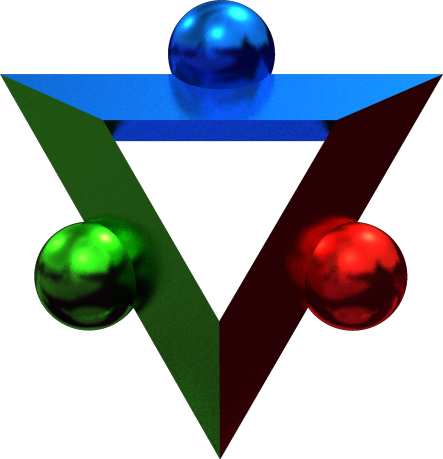
\includegraphics{figure/imudges.png}
                \figcaption{内蒙古大学精英学生开发者联盟}
                \label{fig:emblem} 
            \end{minipage}
        \\[\intextsep] 

        不仅可以并排显示两张图片,还可以图片和表格混排,例如有这样的代码:
        \lstinputlisting[
            caption=一行多图
        ]{codes/figure_table_fix.tex}

        将该代码插入到文档中,可以实现以下图表混排的效果:
        \\[\intextsep] 
            \begin{minipage}{0.5\textwidth} 
                \centering
                
\includegraphics{figure/emblem.png}
                \figcaption{内蒙古大学校徽}
                \label{fig:emblem} 
            \end{minipage}
            \begin{minipage}{0.5\textwidth}
                \centering 
                \begin{tabular}{|c|c|c|}
                    \hline
                        排行 & 编程语言 & 市场占有率 \\
                    \hline
                        1 & C & 17.631\%    \\
                        2 & Java & 17.348\% \\
                        3 & Objective-C & 12.875\% \\
                        4 & C++ & 6.137\% \\
                        5 & C\# & 4.820\% \\
                        6 & (Visual) Basic & 3.441\% \\
                        7 & PHP & 2.773\% \\
                    \hline
                \end{tabular}
                \tabcaption{2014年4月 TIOBE 编程语言排行}
                \label{tab:presidents}
            \end{minipage}
        \\[\intextsep] 

    \section{参考文献}
        本模板\emph{强烈}建议使用BibTex作为文献管理工具。
        模板使用chinesebst作为BibTex文献格式,支持期刊文章、学位论文、专著等格式。
        为了符合国家标准,我们在chinesebst中稍做修改,但不保证chinesebst能够完全符合要求\footnote{But it still works well}。

        BibTex文件以“.bib”结尾,其文件格式和使用方式并未发生改变,所以在此恕不阐述。详细信息可以查看本文档的文献文件“paper.bib”。

        注:此处可以使用本模板定义的命令:\tbs supercite{}来引证文献,可以达到右上角上标显示。例如有如下文段\footnote{摘录自作者本科毕业论文,仅供此文档示例使用,严禁转载!}:

        \subsection{引用文献示例}
            \subsubsection{文段1}
                交互设计是定义、设计人造系统的行为的设计领域\supercite{book_interaction_design}。它结合了“数字媒体”、“人机交互”、“工业设计”、“用户心理学”等多个学科。随着计算机运算性能和增长,人们不再满足于以传统的键盘鼠标作为与计算机交流接口的交互方式。“语音控制”、“意念控制”、“手势控制”等诸多的交互方法已经逐渐走入我们的生活之中。

            \subsubsection{文段2}
                经过查阅相关文献,现在国内的交互设计领域更多的是针对交互内容的优化而鲜有交互方式的变化,例如陈高伟曾经讨论过在线交互设计的现状\supercite{article_current_situation_and_trend_of_design_of_online_interaction},张学军等曾经讨论过交互设计在Flash中应用\supercite{article_flash_interaction_design},卫兵曾研究过基于脑电波的人机交互系统\supercite{thesis_design_and_research_of_a_hci_control_system_based_on_eeg_alpha_reythm},倪晨等曾讨论过Kinect在人机交互领域的应用\supercite{article_the_research_and_application_of_kinect_technology_in_the_field_of_human_computer_interaction}。



        

	
	% 结论
	\include{chapters/conclusion}
	
	% 致谢
	\include{chapters/thanks}

	%参考文献
	\bibliographystyle{chinesebst}	%使用chinesebst
	\bibliography{paper.bib}
	
\end{document}

